\documentclass[tikz,border=22pt]{standalone}
\usepackage[T1]{fontenc}
\usepackage{helvet}
\renewcommand{\familydefault}{\sfdefault}
\usepackage{amsmath,amssymb}
\usetikzlibrary{calc,positioning,fit,backgrounds,shapes.geometric,shapes.symbols,arrows.meta,decorations.pathreplacing}

% =============================================================================
% CANONICAL MLSYSBOOK PALETTE
% =============================================================================
\definecolor{DarkSlate}{HTML}{0F172A}
\definecolor{slatesteel}{HTML}{334155}
\definecolor{BlueLine}{HTML}{006395}
\definecolor{BlueL}{RGB}{209,243,255}
\definecolor{BlueL0}{HTML}{F0F9FF}
\definecolor{BlueDD}{RGB}{20,50,80}
\definecolor{GreenLine}{HTML}{008F45}
\definecolor{GreenL}{RGB}{219,253,166}
\definecolor{GreenL0}{HTML}{EBF8F2}
\definecolor{forestsage}{HTML}{166534}
\definecolor{OrangeLine}{HTML}{E67817}
\definecolor{OrangeL}{RGB}{254,237,222}
\definecolor{OrangeL0}{HTML}{FFFBEB}
\definecolor{warmochre}{HTML}{92400E}
\definecolor{RedLine}{HTML}{D9534F}
\definecolor{RedL}{RGB}{253,226,240}
\definecolor{RedL0}{HTML}{FEF2F2}
\definecolor{deepburgundy}{HTML}{991B1B}
\definecolor{VioletLine}{HTML}{7E317B}
\definecolor{VioletL}{RGB}{247,215,247}
\definecolor{amethyst}{HTML}{581C87}
\definecolor{amethystL0}{HTML}{FAF5FF}
\definecolor{GrayLine}{HTML}{64748B}
\definecolor{coolparchment}{HTML}{F8FAFC}
\definecolor{CardBorder}{HTML}{CBD5E1}
\definecolor{ChipBlack}{HTML}{181F2C}
\definecolor{GoldPin}{HTML}{EAB308}

\tikzset{
  >=Latex,
  font=\sffamily,
  flow_arrow/.style={->, >=Latex, line width=1.3pt},
  flow_arrow_thick/.style={->, >=Latex, line width=1.8pt},
  bus_arrow/.style={<->, >=Latex, line width=2.0pt},
}

\begin{document}
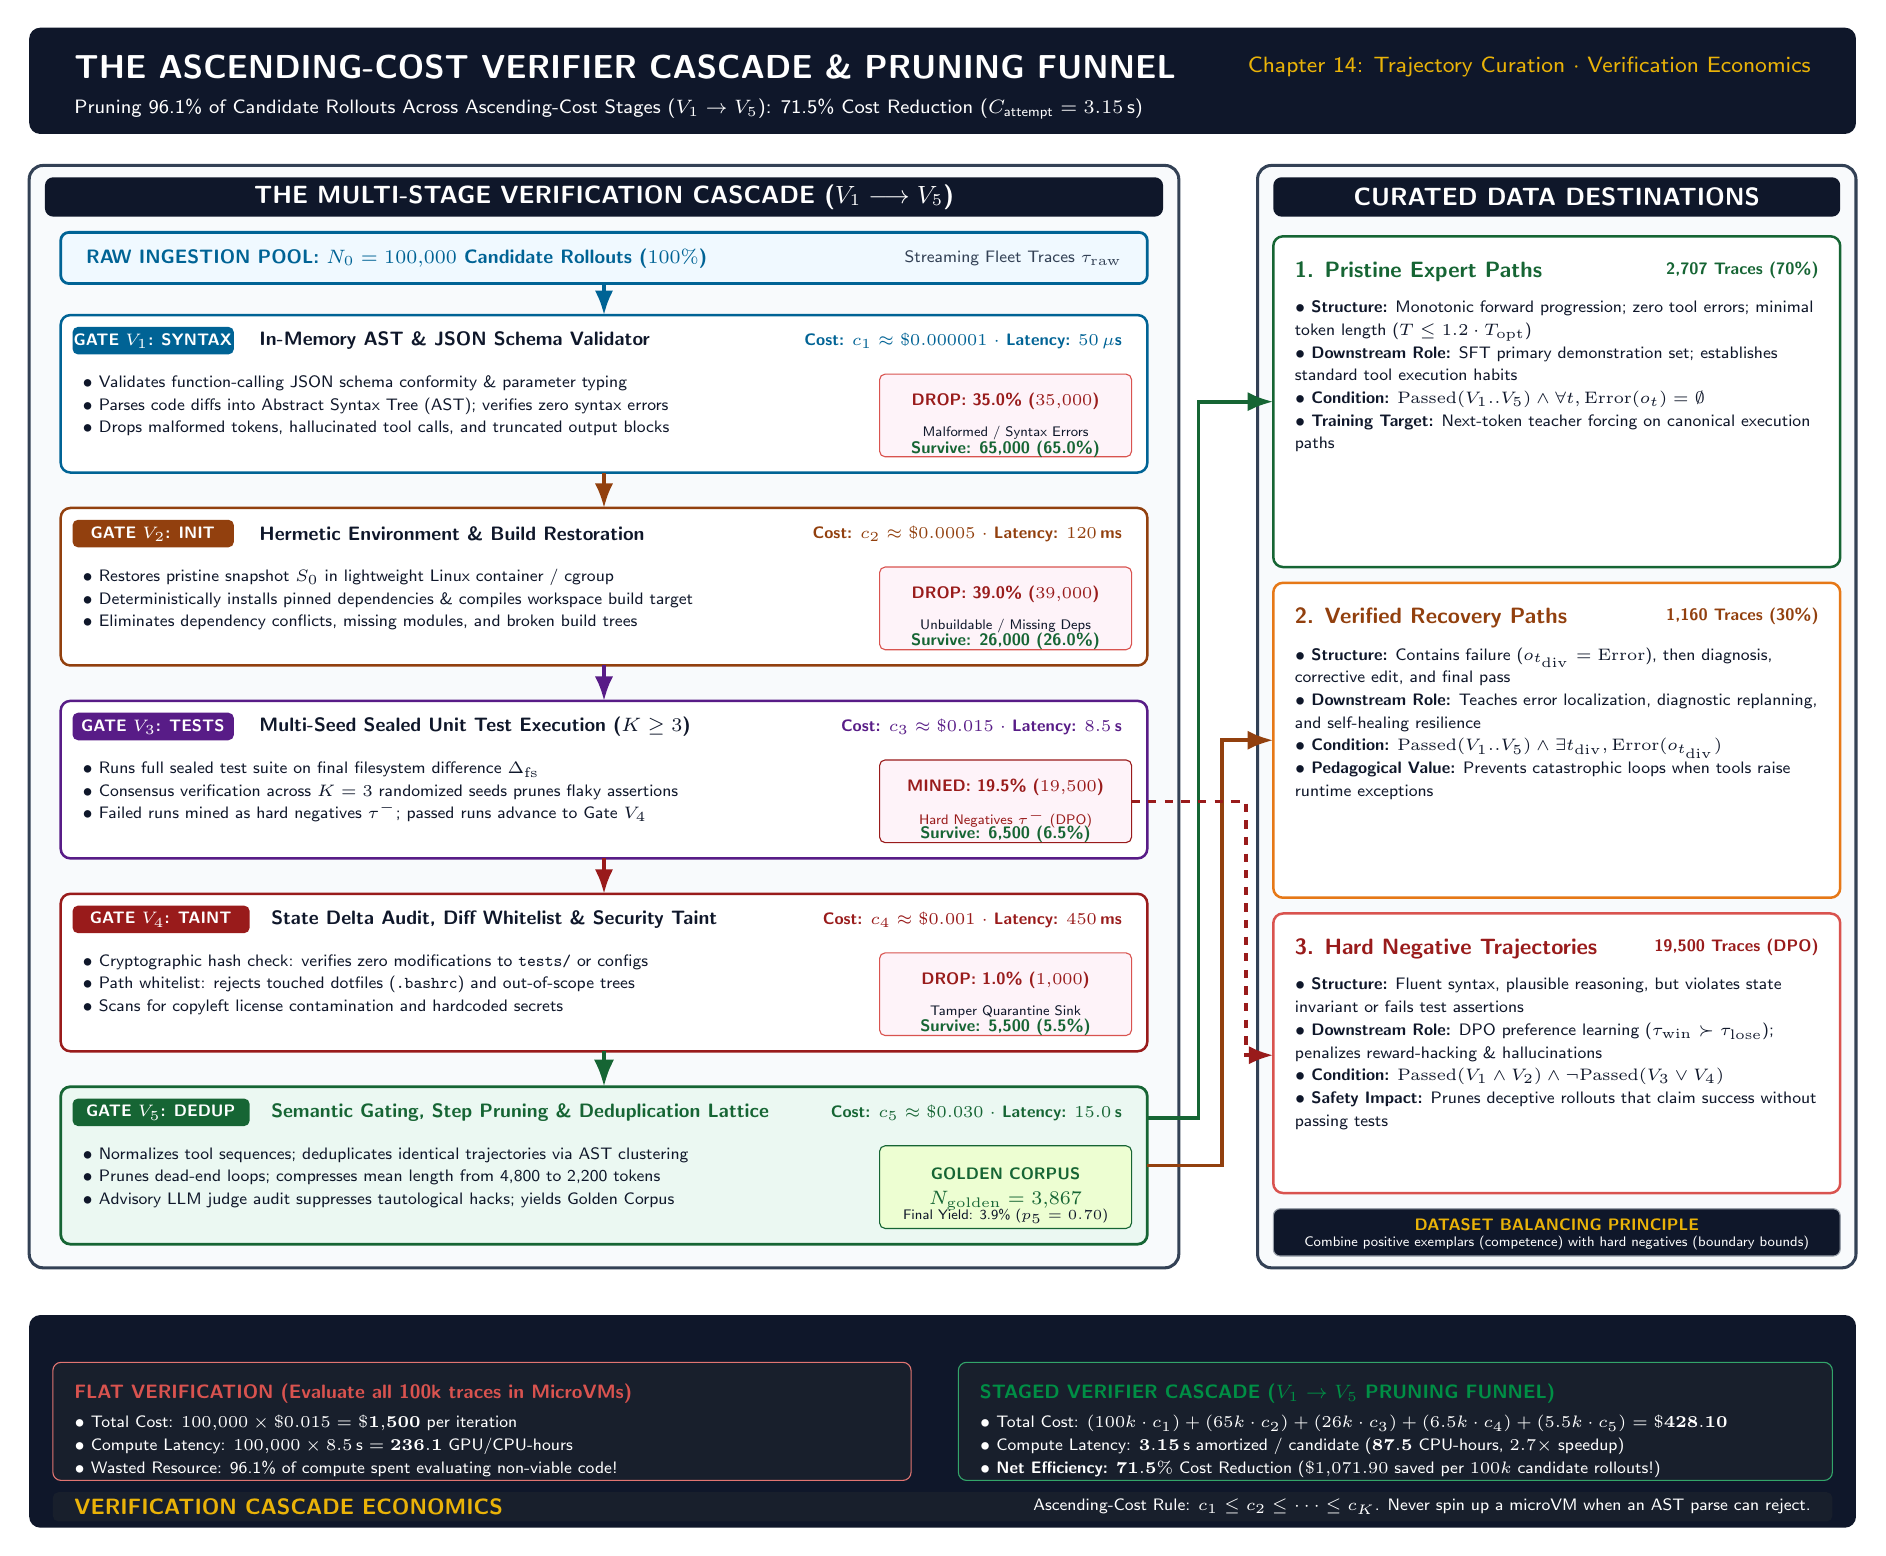
\begin{tikzpicture}[x=1cm, y=1cm]

% =============================================================================
% TOP TITLE BANNER (y: 18.2 to 19.55)
% =============================================================================
\draw[fill=DarkSlate, draw=none, rounded corners=4pt] (0, 18.2) rectangle (23.2, 19.55);
\node[anchor=west, font=\bfseries\large, text=white] at (0.45, 19.05) {
  THE ASCENDING-COST VERIFIER CASCADE \& PRUNING FUNNEL
};
\node[anchor=east, font=\footnotesize, text=GoldPin] at (22.75, 19.05) {
  Chapter 14: Trajectory Curation $\cdot$ Verification Economics
};% Top Subtitle
\node[anchor=west, font=\scriptsize, text=white!85] at (0.45, 18.52) {
  Pruning 96.1\% of Candidate Rollouts Across Ascending-Cost Stages ($V_1 \to V_5$): 71.5\% Cost Reduction ($C_{\text{attempt}} = 3.15\,\text{s}$)
};

% =============================================================================
% 1. LEFT MAIN COLUMN: THE 5-STAGE CASCADING PRUNING FUNNEL
% (x: 0 to 14.6, y: 3.8 to 17.8) - Width 14.6 cm
% =============================================================================
\draw[draw=slatesteel, fill=coolparchment, line width=1.1pt, rounded corners=5pt] (0, 3.8) rectangle (14.6, 17.8);

% Header Bar
\fill[DarkSlate, rounded corners=3pt] (0.2, 17.15) rectangle (14.4, 17.65);
\node[font=\bfseries\small, text=white] at (7.3, 17.4) {
  THE MULTI-STAGE VERIFICATION CASCADE ($V_1 \longrightarrow V_5$)
};

% Raw Ingestion Input Badge (Top of Funnel)
\draw[draw=BlueLine, fill=BlueL0, line width=1.0pt, rounded corners=3pt] (0.4, 16.3) rectangle (14.2, 16.95);
\node[anchor=west, font=\bfseries\scriptsize, text=BlueLine] at (0.6, 16.62) {
  RAW INGESTION POOL: $N_0 = 100{,}000$ Candidate Rollouts ($100\%$)
};
\node[anchor=east, font=\fontsize{6.5pt}{7.5pt}\selectfont, text=slatesteel] at (14.0, 16.62) {
  Streaming Fleet Traces $\tau_{\mathrm{raw}}$
};

% --- STAGE 1: V1 SYNTAX & SCHEMA (y: 13.9 to 15.9) ---
\draw[draw=BlueLine, fill=white, line width=0.9pt, rounded corners=3.5pt] (0.4, 13.9) rectangle (14.2, 15.9);
% Badge
\fill[BlueLine, rounded corners=2pt] (0.55, 15.4) rectangle (2.6, 15.75);
\node[font=\bfseries\fontsize{6.5pt}{7.5pt}\selectfont, text=white] at (1.57, 15.57) {GATE $V_1$: SYNTAX};
\node[anchor=west, font=\bfseries\scriptsize, text=DarkSlate] at (2.8, 15.57) {In-Memory AST \& JSON Schema Validator};
\node[anchor=east, font=\bfseries\fontsize{6.5pt}{7.5pt}\selectfont, text=BlueLine] at (14.0, 15.57) {Cost: $c_1 \approx \$0.000001$ $\cdot$ Latency: $50\,\mu\text{s}$};

\node[anchor=north west, font=\fontsize{6.5pt}{8.2pt}\selectfont, text=DarkSlate] at (0.55, 15.25) {
  \begin{minipage}{9.8cm}\raggedright
    $\bullet$ Validates function-calling JSON schema conformity \& parameter typing\\
    $\bullet$ Parses code diffs into Abstract Syntax Tree (AST); verifies zero syntax errors\\
    $\bullet$ Drops malformed tokens, hallucinated tool calls, and truncated output blocks
  \end{minipage}
};
% Drop Badge
\draw[draw=RedLine, fill=RedL!40, rounded corners=2pt] (10.8, 14.1) rectangle (14.0, 15.15);
\node[font=\bfseries\fontsize{6pt}{7pt}\selectfont, text=deepburgundy] at (12.4, 14.8) {DROP: 35.0\% ($35{,}000$)};
\node[font=\fontsize{5.5pt}{6.5pt}\selectfont, text=DarkSlate] at (12.4, 14.4) {Malformed / Syntax Errors};
\node[font=\bfseries\fontsize{6.5pt}{7.5pt}\selectfont, text=forestsage] at (12.4, 14.2) {Survive: 65,000 (65.0\%)};

% --- STAGE 2: V2 SANDBOX RESTORATION (y: 11.45 to 13.45) ---
\draw[draw=warmochre, fill=white, line width=0.9pt, rounded corners=3.5pt] (0.4, 11.45) rectangle (14.2, 13.45);
\fill[warmochre, rounded corners=2pt] (0.55, 12.95) rectangle (2.6, 13.3);
\node[font=\bfseries\fontsize{6.5pt}{7.5pt}\selectfont, text=white] at (1.57, 13.12) {GATE $V_2$: INIT};
\node[anchor=west, font=\bfseries\scriptsize, text=DarkSlate] at (2.8, 13.12) {Hermetic Environment \& Build Restoration};
\node[anchor=east, font=\bfseries\fontsize{6.5pt}{7.5pt}\selectfont, text=warmochre] at (14.0, 13.12) {Cost: $c_2 \approx \$0.0005$ $\cdot$ Latency: $120\,\text{ms}$};

\node[anchor=north west, font=\fontsize{6.5pt}{8.2pt}\selectfont, text=DarkSlate] at (0.55, 12.8) {
  \begin{minipage}{9.8cm}\raggedright
    $\bullet$ Restores pristine snapshot $S_0$ in lightweight Linux container / cgroup\\
    $\bullet$ Deterministically installs pinned dependencies \& compiles workspace build target\\
    $\bullet$ Eliminates dependency conflicts, missing modules, and broken build trees
  \end{minipage}
};
% Drop Badge
\draw[draw=RedLine, fill=RedL!40, rounded corners=2pt] (10.8, 11.65) rectangle (14.0, 12.7);
\node[font=\bfseries\fontsize{6pt}{7pt}\selectfont, text=deepburgundy] at (12.4, 12.35) {DROP: 39.0\% ($39{,}000$)};
\node[font=\fontsize{5.5pt}{6.5pt}\selectfont, text=DarkSlate] at (12.4, 11.95) {Unbuildable / Missing Deps};
\node[font=\bfseries\fontsize{6.5pt}{7.5pt}\selectfont, text=forestsage] at (12.4, 11.75) {Survive: 26,000 (26.0\%)};

% --- STAGE 3: V3 UNIT & REGRESSION TESTS (y: 9.0 to 11.0) ---
\draw[draw=amethyst, fill=white, line width=0.9pt, rounded corners=3.5pt] (0.4, 9.0) rectangle (14.2, 11.0);
\fill[amethyst, rounded corners=2pt] (0.55, 10.5) rectangle (2.6, 10.85);
\node[font=\bfseries\fontsize{6.5pt}{7.5pt}\selectfont, text=white] at (1.57, 10.67) {GATE $V_3$: TESTS};
\node[anchor=west, font=\bfseries\scriptsize, text=DarkSlate] at (2.8, 10.67) {Multi-Seed Sealed Unit Test Execution ($K \ge 3$)};
\node[anchor=east, font=\bfseries\fontsize{6.5pt}{7.5pt}\selectfont, text=amethyst] at (14.0, 10.67) {Cost: $c_3 \approx \$0.015$ $\cdot$ Latency: $8.5\,\text{s}$};

\node[anchor=north west, font=\fontsize{6.5pt}{8.2pt}\selectfont, text=DarkSlate] at (0.55, 10.35) {
  \begin{minipage}{9.8cm}\raggedright
    $\bullet$ Runs full sealed test suite on final filesystem difference $\Delta_{\mathrm{fs}}$\\
    $\bullet$ Consensus verification across $K=3$ randomized seeds prunes flaky assertions\\
    $\bullet$ Failed runs mined as hard negatives $\tau^-$; passed runs advance to Gate $V_4$
  \end{minipage}
};
% Drop Badge
\draw[draw=deepburgundy, fill=RedL!40, rounded corners=2pt] (10.8, 9.2) rectangle (14.0, 10.25);
\node[font=\bfseries\fontsize{6pt}{7pt}\selectfont, text=deepburgundy] at (12.4, 9.9) {MINED: 19.5\% ($19{,}500$)};
\node[font=\fontsize{5.5pt}{6.5pt}\selectfont, text=deepburgundy] at (12.4, 9.5) {Hard Negatives $\tau^-$ (DPO)};
\node[font=\bfseries\fontsize{6.5pt}{7.5pt}\selectfont, text=forestsage] at (12.4, 9.3) {Survive: 6,500 (6.5\%)};

% --- STAGE 4: V4 INVARIANT & TAINT (y: 6.55 to 8.55) ---
\draw[draw=deepburgundy, fill=white, line width=0.9pt, rounded corners=3.5pt] (0.4, 6.55) rectangle (14.2, 8.55);
\fill[deepburgundy, rounded corners=2pt] (0.55, 8.05) rectangle (2.8, 8.4);
\node[font=\bfseries\fontsize{6.5pt}{7.5pt}\selectfont, text=white] at (1.67, 8.22) {GATE $V_4$: TAINT};
\node[anchor=west, font=\bfseries\scriptsize, text=DarkSlate] at (2.95, 8.22) {State Delta Audit, Diff Whitelist \& Security Taint};
\node[anchor=east, font=\bfseries\fontsize{6.5pt}{7.5pt}\selectfont, text=deepburgundy] at (14.0, 8.22) {Cost: $c_4 \approx \$0.001$ $\cdot$ Latency: $450\,\text{ms}$};

\node[anchor=north west, font=\fontsize{6.5pt}{8.2pt}\selectfont, text=DarkSlate] at (0.55, 7.9) {
  \begin{minipage}{9.8cm}\raggedright
    $\bullet$ Cryptographic hash check: verifies zero modifications to \texttt{tests/} or configs\\
    $\bullet$ Path whitelist: rejects touched dotfiles (\texttt{.bashrc}) and out-of-scope trees\\
    $\bullet$ Scans for copyleft license contamination and hardcoded secrets
  \end{minipage}
};
% Drop Badge
\draw[draw=RedLine, fill=RedL!40, rounded corners=2pt] (10.8, 6.75) rectangle (14.0, 7.8);
\node[font=\bfseries\fontsize{6pt}{7pt}\selectfont, text=deepburgundy] at (12.4, 7.45) {DROP: 1.0\% ($1{,}000$)};
\node[font=\fontsize{5.5pt}{6.5pt}\selectfont, text=DarkSlate] at (12.4, 7.05) {Tamper Quarantine Sink};
\node[font=\bfseries\fontsize{6.5pt}{7.5pt}\selectfont, text=forestsage] at (12.4, 6.85) {Survive: 5,500 (5.5\%)};

% --- STAGE 5: V5 QUALITY & DEDUP (y: 4.1 to 6.1) ---
\draw[draw=forestsage, fill=GreenL0, line width=1.0pt, rounded corners=3.5pt] (0.4, 4.1) rectangle (14.2, 6.1);
\fill[forestsage, rounded corners=2pt] (0.55, 5.6) rectangle (2.8, 5.95);
\node[font=\bfseries\fontsize{6.5pt}{7.5pt}\selectfont, text=white] at (1.67, 5.77) {GATE $V_5$: DEDUP};
\node[anchor=west, font=\bfseries\scriptsize, text=forestsage] at (2.95, 5.77) {Semantic Gating, Step Pruning \& Deduplication Lattice};
\node[anchor=east, font=\bfseries\fontsize{6.5pt}{7.5pt}\selectfont, text=forestsage] at (14.0, 5.77) {Cost: $c_5 \approx \$0.030$ $\cdot$ Latency: $15.0\,\text{s}$};

\node[anchor=north west, font=\fontsize{6.5pt}{8.2pt}\selectfont, text=DarkSlate] at (0.55, 5.45) {
  \begin{minipage}{9.8cm}\raggedright
    $\bullet$ Normalizes tool sequences; deduplicates identical trajectories via AST clustering\\
    $\bullet$ Prunes dead-end loops; compresses mean length from 4,800 to 2,200 tokens\\
    $\bullet$ Advisory LLM judge audit suppresses tautological hacks; yields Golden Corpus
  \end{minipage}
};
% Final Accepted Badge
\draw[draw=forestsage, fill=GreenL!50, rounded corners=2pt] (10.8, 4.3) rectangle (14.0, 5.35);
\node[font=\bfseries\fontsize{6pt}{7pt}\selectfont, text=forestsage] at (12.4, 5.0) {GOLDEN CORPUS};
\node[font=\bfseries\fontsize{7pt}{8pt}\selectfont, text=forestsage] at (12.4, 4.65) {$N_{\mathrm{golden}} = 3{,}867$};
\node[font=\fontsize{5.5pt}{6.5pt}\selectfont, text=DarkSlate] at (12.4, 4.45) {Final Yield: 3.9\% ($p_5=0.70$)};

% Funnel Arrows inside Left Container
\draw[flow_arrow, draw=BlueLine] (7.3, 16.3) -- (7.3, 15.9);
\draw[flow_arrow, draw=warmochre] (7.3, 13.9) -- (7.3, 13.45);
\draw[flow_arrow, draw=amethyst] (7.3, 11.45) -- (7.3, 11.0);
\draw[flow_arrow, draw=deepburgundy] (7.3, 9.0) -- (7.3, 8.55);
\draw[flow_arrow, draw=forestsage, line width=1.5pt] (7.3, 6.55) -- (7.3, 6.1);

% =============================================================================
% 2. RIGHT COLUMN: TAXONOMY OF CURATED TRAJECTORY ROLES
% (x: 15.6 to 23.2, y: 3.8 to 17.8) - Width 7.6 cm
% =============================================================================
\draw[draw=slatesteel, fill=coolparchment, line width=1.1pt, rounded corners=5pt] (15.6, 3.8) rectangle (23.2, 17.8);

% Header Bar
\fill[DarkSlate, rounded corners=3pt] (15.8, 17.15) rectangle (23.0, 17.65);
\node[font=\bfseries\small, text=white] at (19.4, 17.4) {
  CURATED DATA DESTINATIONS
};

% Card 1: Pristine Expert Paths (y: 12.7 to 16.9)
\draw[draw=forestsage, fill=white, line width=0.9pt, rounded corners=3.5pt] (15.8, 12.7) rectangle (23.0, 16.9);
\node[anchor=north west, font=\bfseries\footnotesize, text=forestsage] at (15.95, 16.7) {1. Pristine Expert Paths};
\node[anchor=north east, font=\bfseries\fontsize{6.5pt}{7.5pt}\selectfont, text=forestsage] at (22.85, 16.7) {2,707 Traces (70\%)};
\node[anchor=north west, font=\fontsize{6.5pt}{8.2pt}\selectfont, text=DarkSlate] at (15.95, 16.2) {
  \begin{minipage}{6.7cm}\raggedright
    $\bullet$ \textbf{Structure:} Monotonic forward progression; zero tool errors; minimal token length ($T \le 1.2 \cdot T_{\mathrm{opt}}$)\\
    $\bullet$ \textbf{Downstream Role:} SFT primary demonstration set; establishes standard tool execution habits\\
    $\bullet$ \textbf{Condition:} $\mathrm{Passed}(V_1..V_5) \land \forall t, \mathrm{Error}(o_t) = \emptyset$\\
    $\bullet$ \textbf{Training Target:} Next-token teacher forcing on canonical execution paths
  \end{minipage}
};

% Card 2: Verified Recovery Paths (y: 8.5 to 12.5)
\draw[draw=OrangeLine, fill=white, line width=0.9pt, rounded corners=3.5pt] (15.8, 8.5) rectangle (23.0, 12.5);
\node[anchor=north west, font=\bfseries\footnotesize, text=warmochre] at (15.95, 12.3) {2. Verified Recovery Paths};
\node[anchor=north east, font=\bfseries\fontsize{6.5pt}{7.5pt}\selectfont, text=warmochre] at (22.85, 12.3) {1,160 Traces (30\%)};
\node[anchor=north west, font=\fontsize{6.5pt}{8.2pt}\selectfont, text=DarkSlate] at (15.95, 11.8) {
  \begin{minipage}{6.7cm}\raggedright
    $\bullet$ \textbf{Structure:} Contains failure ($o_{t_{\mathrm{div}}}=\mathrm{Error}$), then diagnosis, corrective edit, and final pass\\
    $\bullet$ \textbf{Downstream Role:} Teaches error localization, diagnostic replanning, and self-healing resilience\\
    $\bullet$ \textbf{Condition:} $\mathrm{Passed}(V_1..V_5) \land \exists t_{\mathrm{div}}, \mathrm{Error}(o_{t_{\mathrm{div}}})$\\
    $\bullet$ \textbf{Pedagogical Value:} Prevents catastrophic loops when tools raise runtime exceptions
  \end{minipage}
};

% Card 3: Hard Negative Contrastive Pairs (y: 4.75 to 8.3)
\draw[draw=RedLine, fill=white, line width=0.9pt, rounded corners=3.5pt] (15.8, 4.75) rectangle (23.0, 8.3);
\node[anchor=north west, font=\bfseries\footnotesize, text=deepburgundy] at (15.95, 8.1) {3. Hard Negative Trajectories};
\node[anchor=north east, font=\bfseries\fontsize{6.5pt}{7.5pt}\selectfont, text=deepburgundy] at (22.85, 8.1) {19,500 Traces (DPO)};
\node[anchor=north west, font=\fontsize{6.5pt}{8.2pt}\selectfont, text=DarkSlate] at (15.95, 7.6) {
  \begin{minipage}{6.7cm}\raggedright
    $\bullet$ \textbf{Structure:} Fluent syntax, plausible reasoning, but violates state invariant or fails test assertions\\
    $\bullet$ \textbf{Downstream Role:} DPO preference learning ($\tau_{\mathrm{win}} \succ \tau_{\mathrm{lose}}$); penalizes reward-hacking \& hallucinations\\
    $\bullet$ \textbf{Condition:} $\mathrm{Passed}(V_1 \land V_2) \land \neg\mathrm{Passed}(V_3 \lor V_4)$\\
    $\bullet$ \textbf{Safety Impact:} Prunes deceptive rollouts that claim success without passing tests
  \end{minipage}
};

% Bottom Takeaway Strip (y: 3.95 to 4.55)
\draw[draw=slatesteel!50, fill=DarkSlate, rounded corners=2.5pt] (15.8, 3.95) rectangle (23.0, 4.55);
\node[font=\bfseries\fontsize{6pt}{7.2pt}\selectfont, text=GoldPin] at (19.4, 4.35) {DATASET BALANCING PRINCIPLE};
\node[font=\fontsize{5.5pt}{6.5pt}\selectfont, text=white!90] at (19.4, 4.12) {Combine positive exemplars (competence) with hard negatives (boundary bounds)};

% Inter-column Arrows from Stage 5 to Data Destinations
% Green line to Card 1: track x = 14.85
\draw[flow_arrow, draw=forestsage, line width=1.4pt] 
  (14.2, 5.7) -- (14.85, 5.7) -- (14.85, 14.8) -- (15.8, 14.8);

% Orange line to Card 2: track x = 15.15
\draw[flow_arrow, draw=warmochre, line width=1.4pt] 
  (14.2, 5.1) -- (15.15, 5.1) -- (15.15, 10.5) -- (15.8, 10.5);

% Red dashed line from Gate V3 drop (y=9.72) to Card 3: track x = 15.45
\draw[flow_arrow, draw=deepburgundy, dashed, line width=1.3pt] 
  (14.0, 9.72) -- (15.45, 9.72) -- (15.45, 6.5) -- (15.8, 6.5);

% =============================================================================
% 3. BOTTOM TIER: VERIFICATION ECONOMICS COMPARISON
% (x: 0 to 23.2, y: 0.5 to 3.2)
% =============================================================================
\draw[fill=DarkSlate, draw=none, rounded corners=4pt] (0, 0.5) rectangle (23.2, 3.2);

% Left Box: Flat Verification Architecture (Anti-pattern)
\draw[draw=RedLine!80, fill=ChipBlack, rounded corners=3pt] (0.3, 1.1) rectangle (11.2, 2.6);
\node[anchor=north west, font=\bfseries\scriptsize, text=RedLine] at (0.45, 2.45) {FLAT VERIFICATION (Evaluate all 100k traces in MicroVMs)};
\node[anchor=north west, font=\fontsize{6.5pt}{8.2pt}\selectfont, text=white!85] at (0.45, 2.05) {
  \begin{minipage}{10.5cm}\raggedright
    $\bullet$ Total Cost: $100{,}000 \times \$0.015 = \mathbf{\$1{,}500}$ per iteration\\
    $\bullet$ Compute Latency: $100{,}000 \times 8.5\,\text{s} = \mathbf{236.1\text{ GPU/CPU-hours}}$\\
    $\bullet$ Wasted Resource: 96.1\% of compute spent evaluating non-viable code!
  \end{minipage}
};

% Right Box: Cascaded Verification Architecture (MLSys Standard)
\draw[draw=GreenLine!80, fill=ChipBlack, rounded corners=3pt] (11.8, 1.1) rectangle (22.9, 2.6);
\node[anchor=north west, font=\bfseries\scriptsize, text=GreenLine] at (11.95, 2.45) {STAGED VERIFIER CASCADE ($V_1 \to V_5$ PRUNING FUNNEL)};
\node[anchor=north west, font=\fontsize{6.5pt}{8.2pt}\selectfont, text=white!85] at (11.95, 2.05) {
  \begin{minipage}{10.7cm}\raggedright
    $\bullet$ Total Cost: $(100k \cdot c_1) + (65k \cdot c_2) + (26k \cdot c_3) + (6.5k \cdot c_4) + (5.5k \cdot c_5) = \mathbf{\$428.10}$\\
    $\bullet$ Compute Latency: $\mathbf{3.15\,\text{s}}$ amortized / candidate ($\mathbf{87.5\text{ CPU-hours}}$, $2.7\times$ speedup)\\
    $\bullet$ \textbf{Net Efficiency:} $\mathbf{71.5\%}$ Cost Reduction ($\$1{,}071.90$ saved per $100k$ candidate rollouts!)
  \end{minipage}
};

% Title Strip inside bus at the BOTTOM
\fill[ChipBlack, rounded corners=2pt] (0.3, 0.58) rectangle (22.9, 0.95);
\node[anchor=west, font=\bfseries\footnotesize, text=GoldPin] at (0.45, 0.77) {
  VERIFICATION CASCADE ECONOMICS
};
\node[anchor=east, font=\fontsize{6.5pt}{8pt}\selectfont, text=white!80] at (22.75, 0.77) {
  Ascending-Cost Rule: $c_1 \le c_2 \le \dots \le c_K$. Never spin up a microVM when an AST parse can reject.
};

\end{tikzpicture}
\end{document}
